\documentclass[../../main.tex]{subfiles}
\begin{document}
\graphicspath{{./figures}}
\chapter{Preprocesamiento de los datos adquiridos}\label{cap::preproc}
Las señales externas son muestreadas por el ADC a 65~MSps en un ancho de banda de 25~MHz como se desarrolló en el \cref{sec::planteo-front-end}. Sin embargo, los \textit{beams} de salida poseen un ancho de banda de apenas 25~kHz, de manera que puede reducirse considerablemente tanto el ancho de banda como la tasa de muestreo. Si se lograse centrar el ancho de banda de un  \textit{beam} en banda base por ejemplo, este solo ocuparía $12.5\un{kHz}$. Esto permitiría teóricamente reducir el ancho de banda de trabajo a $12.5\un{kHz}$ y trabajar con una tasa de muestreo ligeramente superior a 25~kSps cumpliendo con el teorema del muestreo. \cite{teorema-del-muestreo}.

Como se dijo en el \cref{sec::planteo-sist-adq}, esta parte del \textit{core} de adquisición se desarrolla en el presente proyecto. Su diseño, implementación y validación se realizaron primero de manera aislada e independiente a lo desarrollado en \cite{proyecto-jose} y, posteriormente, se integró dentro de dicho sistema.

\section{Requerimientos de diseño}
La etapa de preprocesamiento debe ser capaz de seleccionar uno o varios canales de frecuencia de 25~kHz de ancho de banda, a partir de ahora a estos se les llamará \textit{beams} o haces, reservándose el término \textit{canal} para los canales del ADC.

Luego, partiendo de la banda de UHF de 3~MHz de ancho de banda centrada en $18.5\un{MHz}$ tras el submuestreo, debe obtenerse a la salida uno o varios haces de 25~kHz de ancho de banda.

\section{Diseño conceptual}\label{sec::disenio-conceptual-preproc}
Se parte de la señal real ya submuestreada cuyo espectro está cetrado en $\pm 18.5\un{MHz}$ (ver figura \ref{fig::undersampling}) y su módulo  es simétrico respecto a la frecuencia $f = 0$, como se ilustra en la figura \ref{fig::espectro-inicial}. Dentro de cada triángulo en dicho gráfico se encuentran todos los haces de 25~kHz, replicados a ambos lados del espectro. Esto implica una redundancia de información que puede aprovecharse para optimizar la etapa de preprocesamiento.

Se propone entonces trabajar sobre solo una de estas réplicas mediante una mezcla compleja, esto es, una rotación del espectro \unsure{Agregar referencia?} que permita llevar una de las copias mostradas en \ref{fig::espectro-inicial} a banda base. En este caso es indistinto cuál de las copias se selecciona. 

Asumiendo RABG, se tiene en el espectro una densidad de potencia de ruido independiente de la frecuencia. \unsure{En realidad en el modelo la DEP es estrictamente constante, pero eso no es lo que muestro en las figuras}
Tras el corrimiento de una de las réplicas a BB se procede a realizar también un filtrado como se muestra en la figura \ref{fig::espectro-banda-corrida} reduciendo el ancho de banda de trabajo de manera de filtrar gran parte del ruido entrante. Esta es una primera etapa de ganancia de preprocesamiento, la cual se analizó en el \cref{sec::ganancias-por-preproc}. 

Como puede verse en la figura \ref{fig::espectro-banda-corrida} el ancho de banda del filtro debe ser ligeramente superior a $1.5\un{MHz}$ de manera de tolerar el corrimiento Doppler producido durante la pasada del satélite, el cual puede alcanzar corrimientos de hasta $\pm 10\un{kHz}$, como se desarrolla en el apéndice \ref{ap::doppler}.

Una vez aislada una copia de la banda de interés, resta seleccionar el \textit{beam} que quiere recibirse. Esto puede hacerse mediante un procedimiento similiar al recién aplicado. En este caso, la señal es compleja ya que no hay simetría en el módulo del espectro respecto a $f = 0$, es decir que no existe la redundancia de información que existía al hacer la primer mezcla. Esto implica que el sentido en el que se rota el espectro es relevante.

En la figura \ref{fig::espectro-canal} se muestra el módulo del espectro tras realizar una segunda mezcla compleja partiendo de lo mostrado en la figura \ref{fig::espectro-banda-corrida} para trasladar a BB al haz de interés. El rectángulo en línea de puntos que se muestra en dicha figura representa el filtrado que debe aplicarse tras la mezcla, el cual atenuará el resto de la banda junto con la parte de la potencia de ruido que cae por fuera de la banda de interés, obteniéndose así una segunda ganancia de preprocesamiento.

Nuevamente, si bien los haces tienen 25~kHz de ancho de banda, el filtrado debe contemplar un margen para tolerar el corrimiento Doppler (ver apéndice \ref{ap::doppler}).

\figura[0.8]{espectro-inicial}{Ilustración del módulo del espectro a la entrada de la etapa del preprocesamiento. Se tiene la banda de interés sobre un piso de RABG. Se ve que el espectro es simétrico respecto a la frecuencia $f = 0$ ya que se trata de una señal real.}

\figura[0.8]{espectro-banda-corrida}{Módulo del espectro de la banda de interés trasladada a banda base y filtrada.}

\figura[0.8]{espectro-canal}{Módulo del espectro de la banda de interés centrada en el haz de interés tras la segunda mezcla compleja. El rectángulo en línea punteada representa el filtrado que debe aplicarse psoteriormente para atenuar el resto de la banda y el ruido que cae por fuera del ancho de banda del haz de interés.}

\section{Implementación en software}
A modo de primera comprobación del diseño conceptual previo a su implementación en hardware, se hizo una implementación en software \unsure{JQ: no sé si me gusta 'implementación en SW'. Tal vez lo cambiaría por 'Prueba de concepto en SW'} de la etapa de preprocesamiento empleando Python. 
Esta se encuentra en \texttt{Simulaciones/preprocesamiento.ipynb}. 

Partiendo de la señal submuestreada a 65~MSps mostrada en la figura \ref{fig::undersampling} se aplicó un DDC \cite{DDC}, cuyo diagrama de bloques se muestra en la figura \ref{fig::DDC}. 
Este incluye un NCO el cual genera una exponencial compleja para realizar la rotación de espectro en sentido horario a una frecuencia de $18.5\un{MHz}$, de manera de trasladar la banda de $[-20\un{MHz}, -17\un{MHz}]$ a $[-1.5\un{MHz}, 1.5\un{MHz}]$. 

Ya en banda base, el DDC contiene una etapa de filtrado pasabajos, cuya frecuencia de corte se configuró como $f_c = 1.5\un{MHz}$ de manera de capturar toda la banda de interés dentro de la banda de paso del filtro. El filtrado aplicado fue de tipo Butterworth \cite{Butterworth}, sin embargo, el tipo de filtro elegido no tiene mayor relevancia en la presente implementación\unsure{JQ: por qué?}. Los coeficientes del mismo se obtuvieron mediante la función \texttt{butter} \cite{butter} de la librería de SciPy \cite{scipy} y el filtrado propiamente dicho se realizó usando la función \texttt{lfilter} \cite{lfilter} también de la librería de SciPy. 

Por último, el DDC posee una etapa de decimación en la cual se reduce la tasa de muestreo. Para determinar el factor de decimación debe tenerse en cuenta que la tasa de Nyquist \cite{Nyquist-rate} es ahora de 3~MHz, lo cual implica que la tasa actual de muestreo de 65~MSps podría reducirse hasta en un factor $65/3 = 21.66$ aproximadamente. 
No obstante, para esta implementación se eligió un factor de decimación de 10, de manera que la tasa de muestras a la salida del DDC resulta $6.5\un{MSps}$. La salida de este primer DDC se muestra en la figura \ref{fig::DDC-band}.

Teniendo toda la banda de UHF ya en BB, se procede a seleccionar un haz o \textit{beam} como se muestra en la figura \ref{fig::espectro-canal}. 
Para esto se instancia un nuevo DDC, el cual realiza la mezcla compleja para trasladar el haz a banda base, ejecuta un filtrado del haz con una frecuencia de corte de $f_c = 12.5\un{kHz}$\footnote{Al tratarse de una implementación de prueba, no se tuvo en cuenta el corrimiento Doppler. 
De tenerse en cuenta, debería aumentarse la frecuencia de corte del filtro aproximadamente 10~kHz por encima de la actual.} y finalmente una decimación. 
Para esta última se empleo un factor \todo{Agregar factor}. La salida de este segundo DDC se muestra en la figura \ref{fig::DDC-beam}, donde se observa que pudo aislarse un haz de 25~kHz de ancho de banda de manera exitosa.

\figura[0.7]{DDC}{Diagrama de bloques de un \textit{Digital Down Converter} (DDC).}

\begin{figure}[H]
    \centering
    \subcaptionbox{Salida del primer DDC encargado de trasladar la banda de interés a BB, filtrar y luego decimar con un factor 10..\label{fig::DDC-band}}
    {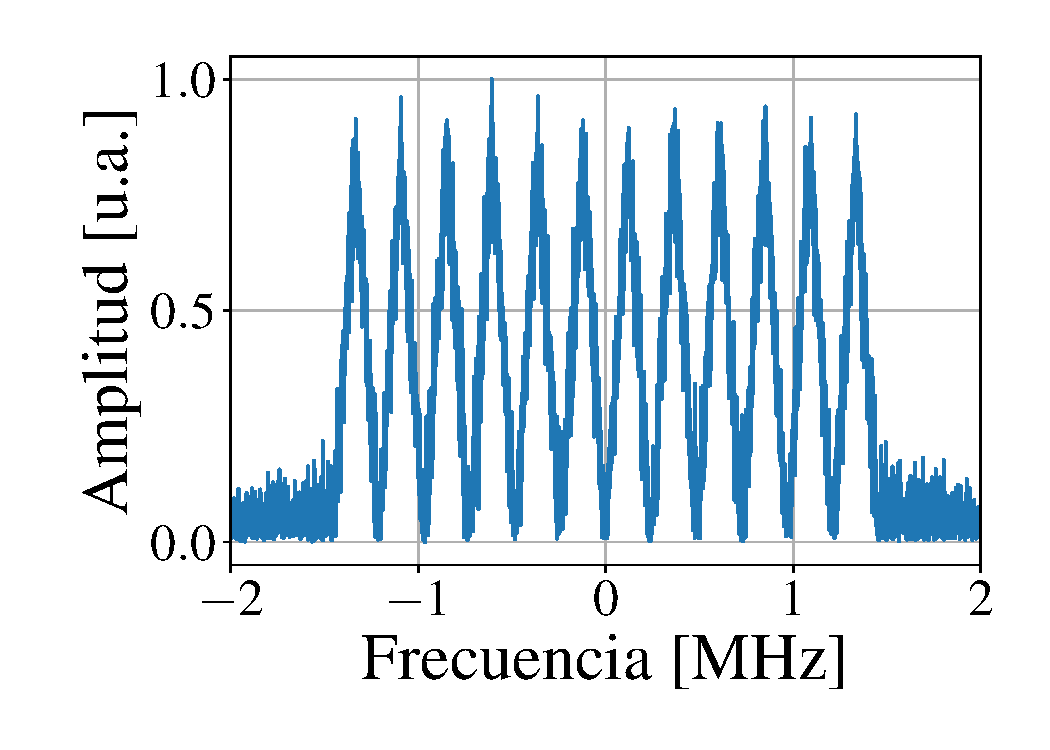
\includegraphics[width=0.49\linewidth]{DDC-band.pdf}}
    \hspace{\fill}%\\[1PC]
    \subcaptionbox{Salida del segundo DDC encargado de seleccionar un \textit{beam}, trasladarlo a BB, filtrarlo y reducir la tasa de muestreo. Se dibuja además una línea vertical en la frecuencia donde termina el canal de interés, esto es, $f = 12.5\un{kHz}$\label{fig::DDC-beam}}
    {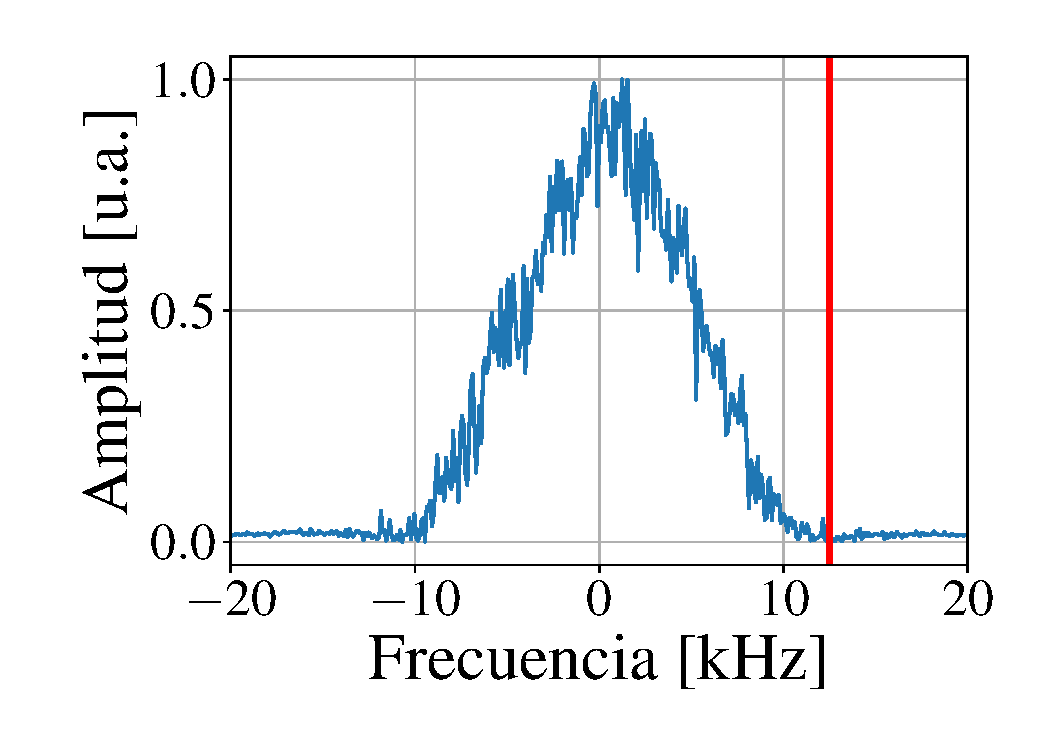
\includegraphics[width=0.49\linewidth]{DDC-beam.pdf}}
    \caption{Salida de las dos etapas de DDCs.}
    \label{fig::DDC-output}
\end{figure}

\section{Implementación en hardware}
Habiendo validado el diseño conceptual mediante una implementación en software se procede a realizar una implementación del mismo en la placa CIAA-ACC. Dado que el SoC Zynq-7030 incluido en la CIAA-ACC es fabricado por la compañía Xilinx, se hizo uso de su entorno de desarrollo, el cual incluye al software \textit{Vivado} \cite{vivado} para el desarrollo, síntesiss e implementación en la FPGA y al software \textit{Vitis Unified Software Platform} \cite{vitis} para el desarrollo y la compilación cruzada \cite{cross-compilation} del software para el PS. La versión del entorno de desarrollo usada en este proyecto fue la 2020.2.

La tasa de muestreo del AD9249 es de 65~MSps como se indica en la tabla \ref{tab::ADC}, esto fija la tasa de datos que tiene que procesar la FPGA y representa una frecuencia mínima de reloj a emplear. En base a esto, se eligió una frecuencia de reloj de 260~MHz para realizar el preprocesamiento de manera de disponer de 4 ciclos de reloj entre cada muestra que entrega el ADC\footnote{$260\un{MHz} = 4 \cdot 65\un{MHz}.$}. Esto puede otorgar cierta flexibilidad a la hora de diseñar el \textit{pipeline} de preprocesamiento.

Esta implementación es de tipo \textit{standalone}, es decir, se hizo de manera aislada al sistema desarrollado en \cite{proyecto-jose} y se consideró un único \textit{beam} de salida como primera prueba de concepto.

Un esquema general con finalidad de servir como guía para la implementación se muestra en la figura \ref{fig::disenio-para-hw}, donde las señales de datos se encuentran en negro y las de control en naranja. En esta figura también se observan las etapas de mezcla y filtrado concebidas en la sección \ref{sec::disenio-conceptual-preproc} junto con los bloques
\begin{itemize}
    \item \texttt{Data source hier}: su objetivo es controlar la fuente de datos que ingresa al preprocesamiento, sobre todo con finalidades de \textit{debug} como se explicará en breve en la subsección \ref{subsec::debug-preproc-inicial}.
    \item \texttt{AXI hier}: este bloque agrupa todo el hardware relacionado a la interconexión con el PS lo cual permitirá controlar la \texttt{Data source hier} mediante registros.
\end{itemize}

\figura[0.85]{disenio-para-hw}{Esquema guía para la implementación de la etapa de preprocesamiento en hardware. Se indican en negro las señales de datos y en naraja las de control.}

\subsection{IPs empleadas}
\textit{Vivado} cuenta con interfaces o bloques propietarios en su librería de propiedad intelectual o IP \cite{IP-Xilinx}. Estos funcionan como caja negra para el usuario, recibiendo entradas y produciendo salidas acordes a su funcionalidad.

En el desarrollo de la etapa de preprocesamiento se utilizaron las IPs de \textit{Vivado} nombradas en la tabla \ref{tab::ip-vivado-preproc}.
\begin{table}[H]
    \centering
    \resizebox{\textwidth}{!}{%
    \begin{tabular}{|llc|}
    \hline
    \multicolumn{3}{|c|}{\textbf{IPs nativas utilizadas}}                                                                                                                                                                                                                                                        \\ \hline
    \multicolumn{1}{|l|}{\textbf{Nombre}}    & \multicolumn{1}{l|}{\textbf{Función}}                                                                                                                                                                                  & \textbf{Documentación}                   \\ \hline
    \multicolumn{1}{|l|}{AXI Interconnect}   & \multicolumn{1}{l|}{\begin{tabular}[c]{@{}l@{}}Conecta uno o más dispositivos maestros AXI mapeados\\ en memoria a uno o más dispositivos esclavos mapeados\\ en memoria.\end{tabular}}                                & \cite{axi-interconnect} \\ \hline
    \multicolumn{1}{|l|}{Complex Multiplier} & \multicolumn{1}{l|}{\begin{tabular}[c]{@{}l@{}}Implementa multiplicadores complejos optimizados, de\\ alto rendimiento y compatibles con AXI4-Stream basados\\ en opciones especificadas por el usuario.\end{tabular}} & \cite{complex-mult}     \\ \hline
    \multicolumn{1}{|l|}{DDS Compiler}       & \multicolumn{1}{l|}{Genera señales sinusoidales.}                                                                                                                                                                      & \cite{dds-compiler}     \\ \hline
    \multicolumn{1}{|l|}{FIR Compiler}       & \multicolumn{1}{l|}{Genera un filtro tipo FIR.}                                                                                                                                                                        & \cite{fir-compiler}     \\ \hline
    \end{tabular}%
    }
    \caption{IPs nativas utilizadas en el desarrollo de la etapa de preprocesamiento.}
    \label{tab::ip-vivado-preproc}
    \end{table}

\subsection{Módulos desarrollados}
Además de emplear IPs de \textit{Vivado}, se desarrollaron módulos en VHDL accesibles en el directorio \texttt{Fpga/prj/preprocessing\_stage/src}. Dichos módulos y su función se mencionan a continuación en la tabla \ref{tab::ip-fran}\todo{JQ: revisar si falta alguno (FIFO input data mux?)}.

La integración de estos módulos con las IPs de Xilinx serán más claras en breve cuando se explique la composición del sistema implementado.

\todo{Incluir Complelx\_gain}
\begin{table}[H]
    \resizebox{\textwidth}{!}{%
    \begin{tabular}{|ll|}
    \hline
    \multicolumn{2}{|c|}{\textbf{Módulos desarrollados}}                                                                                                                                                                                                                                                                                                                                                               \\ \hline
    \multicolumn{1}{|l|}{\textbf{Nombre}}                                                   & \textbf{Función}                                                                                                                                                                                                                                                                                                         \\ \hline
    \multicolumn{1}{|l|}{\begin{tabular}[c]{@{}l@{}}DDS Compiler\\ Controller\end{tabular}} & \begin{tabular}[c]{@{}l@{}}Opera con la interfaz AXI4-Stream. Su entrada es la salida de\\ un DDS Compiler. Mediante el pulso de tready del protocolo\\ AXI4-Stream controla la tasa a la cual el DDS Compiler \\ genera nuevos datos, convirtiendola en cualquier submúltiplo de\\ la frecuencia de reloj.\end{tabular} \\ \hline
    \multicolumn{1}{|l|}{\begin{tabular}[c]{@{}l@{}}Valid Data\\ Holder\end{tabular}}       & \begin{tabular}[c]{@{}l@{}}Opera con la interfaz AXI4-Stream. Sostiene el último dato\\ válido en la salida hasta que llega uno nuevo.\end{tabular}                                                                                                                                                                      \\ \hline
    \multicolumn{1}{|l|}{Basic Counter}                                                     & \begin{tabular}[c]{@{}l@{}}Contador de ancho ajustable que se incrementa cada N \\ ciclos de reloj, con N configurable.\end{tabular}                                                                                                                                                                                     \\ \hline
    \multicolumn{1}{|l|}{Zero Padder}                                                       & \begin{tabular}[c]{@{}l@{}}Convierte una señal de N bits en una de M bits con M\textgreater{}N\\ agregando ceros ya sea a derecha o a izquierda.\end{tabular}                                                                                                                                                            \\ \hline
    \multicolumn{1}{|l|}{Data Source Mux}                                                   & \begin{tabular}[c]{@{}l@{}}Multiplexor con 3 entradas tipo AXI4-Stream y una señal\\ de control.\end{tabular}                                                                                                                                                                                                            \\ \hline
    \multicolumn{1}{|l|}{AXI Slave Reg}                                                     & Bloque de registros que implementan el protocolo AXI4-Lite.                                                                                                                                                                                                                                                              \\ \hline
    \multicolumn{1}{|l|}{CDC Two FF Sync}                                                   & \begin{tabular}[c]{@{}l@{}}Dos FF en serie. Sirven para sincronizar un bit de una señal\\ asíncrona.\end{tabular}                                                                                                                                                                                                        \\ \hline
    \multicolumn{1}{|l|}{CDC Comparator}                                                    & Compara dos entradas y la asigna a la salida en caso de ser iguales.                                                                                                                                                                                                                                                     \\ \hline
    \end{tabular}%
    }
    \caption{Módulos desarrollados en VHDL para el desarrollo de la etapa de preprocesamiento.}
    \label{tab::ip-fran}
    \end{table}

\subsection{Filtros y decimación}\label{subsec::filtros-decimacion}
Según el esquema guía de la figura \ref{fig::disenio-para-hw} y lo desarrollado en \ref{sec::disenio-conceptual-preproc} deben implementarse dos etapas digitales de filtrado pasabajos y decimación, una después de realizar cada mezcla. 

Al diseñar la etapa de filtrado deben tenerse en cuenta las consideraciones habituales \unsure{No mg mucho esa palabra} como la evaluación del tipo de filtro, la frecuencia de corte, el orden del filtro, entre otros. Pero además, al tratarse de un filtro a ser implementado en hardware, debe tenerse en cuenta que el mismo hará uso de aritmética de punto fijo \cite{pto-fijo}. Esto implica que el número de dígitos decimales con los que se trabaja se mantiene constante.

\subsubsection{Diseño de los filtros}
Para el diseño de los filtros se utilizó el programa MATLAB \todo{ref?}, el cual incorpora herramientas tales como \texttt{Filter Builder} \todo{ref} y \texttt{Filter Designer} \todo{ref}. Estas herramientas permiten realizar el diseño de filtros de todo tipo a partir de los parámetros de interés de cada aplicación en particular. 

\texttt{Filter Builder} y \texttt{Filter Designer} también son capaces de trabajar con aritmética de punto fijo y generar el código en VHDL para utilizar directamente en \textit{Vivado}. A priori esta puede ser una opción viable, sin embargo, dado que los filtros se implementarán con el \textit{IP Block} \texttt{FIR Compiler} nativo de Xilinx, no se necesita el código en VHDL. En cambio, el \texttt{FIR Compiler} requiere que se lo configure con los valores de los coeficientes. Para esto se usa un archivo con extensión \textit{coe} que es un archivo de texto indicando los valores de todos los coeficientes, la base numérica en la que están expresados (llamado \textit{radix}) y el ancho en bits de los mismos. Un recorte de un archivo de coeficientes se muestra en la figura \ref{fig::coef-file}. Este recorte corresponde al archivo empleado en la configuración del primer filtro pasabajos.

Resulta relevante destacar que finalmente, a pesar de las capacidades de operación con aritmética de punto fijo que tienen las herramientas de MATLAB, el diseño de los filtros se hizo con aritmética de punto flotante. La razón detrás de esto es que \textit{Vivado}, a través del \texttt{FIR Compiler}, cuenta con su propio método de implementación en punto fijo a partir de punto flotante. Es decir, el \texttt{FIR Compiler} puede configurarse con aritmética de punto flotante y él mismo se encarga de convertirlo a aritmética de punto fijo.

\figura[0.7]{coef-file}{Ejemplo de archivo de configuración generado con MATLAB para el \texttt{FIR Compiler}.}

El primer filtrado se designará a partir de ahora como \textit{filtrado de banda}. Este nombre proviene del hecho de que este es el filtrado a ser aplicado tras la traslación de la banda de interés a BB. Este filtrado debe contener a la banda de interés en su banda de paso. Al estar en BB, la máxima frecuencia de la banda de interés de 3~MHz de ancho de banda es $f_\textrm{max} = 1.5\un{MHz}$. Luego, usando la herramienta \texttt{Filter Designer} se generaron los coeficientes para un filtro FIR pasabajos de tipo equirripple \todo{ref!}. La respuesta del fitro junto con las configuraciones se muestran en la figura \todo{Poner captura de Filter Designer}. Adeamás, sus especificaciones se listan en la tabla \todo{Hacer tabla}

Para el caso del segundo filtrado, a partir de ahora \textit{filtrado de haz}, se opera de forma análoga al anterior. En este caso se tiene el requerimiento de que cada beam tiene alrededor de 25~kHz de ancho de banda \change{En BB es la mitad. De todas formas hay que tener en cuenta Doppler asi que vuelve approx a 25.}. Como una primera iteración se diseñó un filtro de 50~kHz de ancho de banda, cuyas especificaciones se encuentran en la table \todo{hacer tabla, misma que antes?} y su respuesta en frecuencia se ilustra en la figura \todo{Poner captura del filter designer}.


\subsubsection{Tasas de decimación}
Tras el primer filtrado se tiene toda la información de la banda de UHF de interés ahora en el rango de frecuencias $-1.5\un{MHz}<f<1.5\un{MHz}$. De esta manera, se requiere una tasa de muestreo mínima superior a los 3~MHz (\cite{teorema-del-muestreo}). Partiendo de la tasa actual de muestreo de 65~MSps, puede incorporarse un factor de decimación máximo:
\[\textrm{Factor de decimación máximo} = \left\lfloor\frac{65\un{MSps}}{3\un{MSps}}\right\rfloor = 21.\]
Para esta implementación \textit{standalone} se eligió un factor de decimación de 8. Este parámetro es configurable directamente en el \texttt{FIR Compiler}, el cual se encarga de la optimización de recursos \cite{fir-compiler}. Así, la tasa de datos a la salida del filtrado de banda es $f'_s = 8.125\un{MHz}$.

Tras el filtrado de canal se tiene que a la salida el ancho de banda es de 50~kHz. Luego, se requiere una frecuencia de muestreo de al menos 100~kHz. Esto permite tener el siguiente factor máximo de decimación:
\[\textrm{Factor de decimación máximo} = \left\lfloor\frac{8.125\un{MSps}}{100\un{kSps}}\right\rfloor = 81.\] En este caso se eligió una tasa de decimación de 50.

\todo{Figuras y tablas}

\subsection{Herramientas de \textit{debug}}\label{subsec::debug-preproc-inicial}
En todo desarrollo resulta importante incorporar herramientas para poder \textit{debuggear} el sistema cuando algo no esté funcionando. Con este propósito se empleó el módulo \texttt{Data Source Mux} mencionado en la tabla \ref{tab::ip-fran} al cual se conectaron tres entradas:
\begin{itemize}
    \item Los datos del ADC. Este es el modo de operación normal, no de \textit{debug}.
    \item Una instancia del módulo \texttt{Basic Counter} (ver tabla \ref{tab::ip-fran}).
    \item Una instancia del IP \texttt{DDS Compiler} oscilando a una frecuencia conocida y controlado mediante una instancia de \texttt{DDS Compiler Controller} (ver tablas \ref{tab::ip-vivado-preproc} y \ref{tab::ip-fran}).
\end{itemize}

El multiplexor se controla mediante un registro en el módulo \texttt{AXI Slave Reg} conectado a su vez al IP AXI Interconnect.

\subsection{Cruces de dominio de reloj (CDCs)}
Un dominio de reloj se compone de todos los elementos de un circuito lógico que operan bajo la misma señal de \textit{clock}.

Al realizar desarrollo en hardware, una situación que se presenta con regularidad es la necesidad de sincronizar con un dado reloj una señal que proviene de otro dominio de reloj. Esta situación recibe el nombre de \textit{Clock Domain Crossing} (CDC) y debe ser manejada de manera de poder asegurar el cumplimiento de los tiempos de \textit{setup} y \textit{hold} de los \textit{flip-flops} controlados por el nuevo reloj.

En el caso de la señal de control del \texttt{Data Source Mux}, la misma se encuentra dentro del dominio de reloj del AXI Interconnect (el cual generalmente viene dado por el PS). Al tratarse de una señal lenta ya que cambia en tiempos muy largos, puede sincronizarse en el nuevo dominio de reloj (esto es, el de 260~MHz) como si se tratara de una señal asíncrona. Para esto se hace uso del módulo \texttt{CDC Two FF Sync}.

Sin embargo, dicho módulo por si solo se emplea para sincronizar un único bit \todo{referencia?}. En este caso, la señal de control del multiplexor tiene 2 bits (hay 3 entradas), en consecuencia, para asegurar la integridad de la señal en el CDC se emplean dos \texttt{CDC Two FF Sync} en serie y se comparan sus salidas con el módulo \texttt{CDC Comparator} como se muestra en la figura \ref{fig::CDC-preproc}. Si ambas salidas son iguales, entonces la señal se sincroniza exitósamente al dominio de reloj de 260~MHz.

\figura{CDC-preproc}{Sincronizador de 2 bits para señales lentas empleado para realizar el CDC de la señal de control del multiplexor desde el dominio de reloj del AXI Interconnect al dominio de reloj de 260~MHz.}

\subsection{Implementación en \textit{Vivado}}
Haciendo uso e interconectando los bloques de IP de las tablas \ref{tab::ip-vivado-preproc} y \ref{tab::ip-fran} puede implementarse el diseño conceptual descrito en la sección \ref{sec::disenio-conceptual-preproc} tomando comó guía el esquema de la figura \ref{fig::disenio-para-hw}. 

Cabe destacar que el diseño realizado implica trabajar con números complejos ya sea en las mezclas, en los filtros y en toda la cadena de preprocesamiento en general. Como consecuencia de esto se tendrán que realizar las adaptaciones correspondientes, las cuales se describirán oportunamente a medida que surjan naturalmente.

A continuación se aborda la implementación en \textit{Vivado} de este esquema.

\subsubsection{Jerarquía AXI}
La jerarquía AXI (o AXI hier) mostrada como un bloque del flujo de preprocesamiento en la figura \ref{fig::disenio-para-hw} se muestra con mayor detalle en la figura \ref{fig::axi-hier}. La misma se compone de dos \textit{IP blocks}, una instancia del \texttt{AXI Interconnect} conectado a través de una interfaz AXI4-Lite a un \texttt{AXI Slave Reg}. 

El objetivo de esta jerarquía es permitir la comunicación con la FPGA desde el exterior mediante la escritura de registros. En este caso, la señal de control para el \texttt{Data Source Mux} como se aclaró en la subsección \ref{subsec::debug-preproc-inicial}.

\todo{Incorporar mapeo de registros}

\figura[0.85]{axi-hier}{Jerarquía AXI compuesta por un \texttt{AXI Interconnect} y un \texttt{AXI Slave Reg} interconectados a través de una interfaz AXI4-Lite.}

\subsubsection{Data source hier}
Esta jerarquía abarca a toda la lógica relacionada a la selección de los datos de entrada, e incorpora todas las fuentes de señal de \textit{debug} discutidas en la subsección \ref{subsec::debug-preproc-inicial}. El diagrama de bloques de esta jerarquía se muestra en la figura \ref{fig::data-source-hier}. El multiplexor de datos se controla mediante una señal externa, la cual será mapeada a un registro en la interconexión final.

Algunos puntos importantes a notar son los siguientes:
\begin{itemize}
    \item Se incopora una etapa de \textit{zero padding} a derecha (equivalennte a una multiplicación por 4) a la muestra proveniente del ADC ya qua la misma tiene 14 bits, y se neceita extenderla a 16.
    \item El bloque \texttt{Valid Data Holder} en principio no afecta el funcionamiento de la cadena. Sin embargo, su presencia es importante durante simulación para mantener el último dato constante hasta el próximo pulso de \textit{valid}. Esto se explicará mejor en la sección \ref{sec::simu-uvm}.
    \item A la salida de datos del \texttt{Data Source Mux} se le hace un \textit{zero padding} de 16 bits por izquierda. Esto es consecuencia de que se trabajará con números complejos de 32 bits en total, de manera que los primeros 16 bits corresponden a la parte real y los últimos 16 corresponden a la parte imaginaria. Al tratarse de todas señales de entrada reales (tanto las del ADC como las de \textit{debug}), se fija la parte imaginaria en cero al convertir la salida del multiplexor a un número complejo.
    \item La jerarquía \textit{Local\_osc\_hier} instancia un \texttt{DDS Compiler} controlado por un \texttt{DDS Compiler Controller} como se explicó en la subsección \ref{subsec::debug-preproc-inicial}.
\end{itemize}

\figura[0.85]{data-source-hier}{Jerarquía de fuente de datos. La misma incorpora fuentes de \textit{debug} y se controla mediante un registro.}

\subsubsection{Osciladores}
Se instancian en total tres osciladores: uno para funcionar como fuente de datos de \textit{debug}, uno para realizar la primer mezcla o mezcla de banda, y otro para realizar la segunda mezcla o la mezcla de \textit{beam}. Resulta relevante recordar que esta implementación contempla un único \textit{beam}, ya que, si se quisieran obtener N haces a la salida se necesitarían N osciladores, esto es, si no se hace ningún tipo de optimización.

El oscilador de \textit{debug} se conforma de dos \textit{IP Blocks} como se muestra en la figura \ref{fig::local-osc}, estos son:
\begin{itemize}
    \item \texttt{DDS Compiler}: es el encargado de generar la sinusoide a la frecuencia de interés.
    \item \texttt{DDS Compiler Controller}: controla la tasa a la que el DDS Compiler entrega los datos pidiendo los datos a la tasa deseada mediante el uso del pulso de \textit{tready} del protocolo AXI4-Stream.
\end{itemize}

La incorporación del \texttt{DDS Compiler Controller} es necesaria ya que no se encontró otra manera de controlar la tasa de generación de datos del \texttt{DDS Compiler} que no sea a través de la señal \textit{tready} de entrada. Para el caso de los osciladores de banda y de \textit{beam}, el pulso de \textit{tready} está conectado al pulso de \textit{tvalid} de los datos de entrada a los mezcladores.

El \texttt{DDS Compiler} es capaz de generar un coseno puro, un seno puro o una combinación coseno-seno. Esta última es de particular relevancia ya que se corresponde a una exponencial compleja\footnote{Esto es la fórmula de Euler: $e^{j \theta} = \cos(\theta) + j\sen(\theta)$}, lo cual permite realizar las mezclas originalmente concebidas en la sección \ref{sec::disenio-conceptual-preproc}.

Para configurar el ancho de la señal de salida del \texttt{DDS Compiler} debe elegirse la opción \textit{Hardware Parameters} en el campo de \textit{Parameter Selection}. Se configura entonces la señal salida a 16 bits en todos los casos, contemplando que si se le pide que genere una señal tipo exponencial compleja, el ancho será de 32 bits (16 bits para la parte real y 16 para la imaginaria).

La frecuencia del oscilador en el modo de \textit{Hardware Parameters} se elige a través de la escritura en binario del incremento de fase deseado. Para calcular el incremento de fase $\Delta \theta$ correspondiente a una frecuencia de configuración $f_\textrm{conf}$ se utiliza la siguiente fórmula \cite[p. 17]{dds-compiler}:

\begin{equation}
     \Delta \theta = \frac{2^N}{f_\textrm{clk}} f_\textrm{conf},
     \label{eq::calculo-incremento-fase}
\end{equation}
donde $N$ es el número de bits usados en la definición del incremento de fase, en este caso se usó $N = 16$. Esta fórmula se desprende del hecho de que la máxima frecuencia de salida que puede generar el sintetizador es $f_\textrm{clk}$.

Una precaución que debe tenerse, sin embargo, es que al estar controlando la tasa a la que entregan los datos los osciladores mediante la señal de \textit{tready}, la frecuencia efectiva de la señal generada se verá afectada por un factor igual al factor de reducción de datos respecto a la frecuencia de reloj $f_\textrm{clk}$. 
Esto implica que la frecuencia de configuración $f_\textrm{conf}$ solo coincidirá con la frecuencia de salida $f_\textrm{out}$ cuando se desee generar un dato nuevo por ciclo de reloj. 
Es decir, si se quiere por ejemplo obtener una frecuencia de salida $f_\textrm{out} = 18.5\un{MHz}$ muestreada a 65~MSps con un reloj cuatro veces más rápido de $f_\textrm{clk} = 65 \cdot 4 = 260\un{MHz}$ se debe configurar el \texttt{DDS Compiler} para operar a una frecuencia cuatro veces más rápida. En este caso la frecuencia de configuración sería $f_\textrm{conf} = 4 \cdot f_\textrm{out} = 74\un{MHz}$.

De esta manera, reemplazando $f_\textrm{conf}$ por \[f_\textrm{out} = \frac{f_\textrm{datos}}{f_\textrm{clk}}f_\textrm{conf}\] en la ecuación \ref{eq::calculo-incremento-fase} para incluir los casos donde la tasa de generación de datos deseada es menor a la frecuencia del reloj, se obtiene el incremento de fase necesario para obtener una señal de frecuencia efectiva $f_\textrm{out}$ a la salida del DDS.

\begin{equation}
    \Delta \theta = \frac{2^N}{f_\textrm{datos}} \cdot f_\textrm{out} \\
    \label{eq::calculo-incremento-fase-v2}
\end{equation}

Las frecuencias seleccionadas para los osciladores se muestran en la tabla \todo{citar y hacer tabla: Osc - Freq - Modo}. A continuación se justifican estan elecciones:
\begin{itemize}
    \item La frecuencia del oscilador de banda se eligió de manera que la banda submuestreada amateur de UHF quede centrada en BB tras la mezcla.
    \item La frecuencia del oscilador de \textit{beam} se seleccionó de manera arbitraria a modo de demostración con la restricción de que $-1.5\un{MHz}<f<1.5\un{MHz}$, de manera de asegurarse que la salida de la mezcla esté dentro de la banda de interés.
    \item La frecuencia del oscilador local de \textit{debug} se seleccionó en base a las dos anteriores de manera que a la salida de la etapa de preprocesamiento se obtenga una señal visible ya que, tras las dos mezclas, la señal del oscilador local queda en $f = -10\un{kHz}$. Esto es útil para una primera comprobación del funcionamiento del sistema.
\end{itemize}

\figura[0.8]{local-osc}{Ejemplo de uno de los osciladores instanciados en el diseño, en este caso se trata del oscilador de \textit{debug}, el cual incorpora el \texttt{DDS Compiler Oscillator Controller}.}

\subsection{Mezcladores}
Los mezcladores mostrados en la figura \ref{fig::disenio-para-hw} se implementaron usando el IP \texttt{Complex Multiplier}, presentado en la tabla \ref{tab::ip-vivado-preproc}. Este multiplicador implementa el protocolo AXI4-Stream y solo realiza la multiplicación cuando ambas señales de entrada tienen su \textit{tvalid} activo.

Para asegurar que ambos datos sean válidos al mismo tiempo, puede ignorarse la señal de \textit{tvalid} de los osciladores y conectar a ambos puertos una única señal de \textit{tvalid}. Esto es posible ya que no se necesita un sincronismo de fase particular a la hora de comenzar a realizar la multiplicación, ya que la traslación en frecuencia es independiente de la fase inicial del oscilador. 

Una situación que sí es relevante es que el cada muestra del oscilador sea utilizada para realizar la mezcla, ya que saltear muestras implicaría un cambio en la frecuencia efectiva del mismo. 
Para garantizar que los osciladores de banda y de haz generen una única muestra nueva por cada dato nuevo del \textit{pipeline} de datos, se conectó su señal de \textit{tready} a la señal de \textit{tvalid} de los datos. Así, cuando un dato del \textit{pipeline} es válido los osciladores producen un nuevo dato y se realiza la multiplicación.

Al multiplicar dos números de $N\un{bits}$ se obtiene a la salida una señal en \textit{full precision} de $2 N + 1\un{bits}$. No obstante, se truncó la salida a $N$~bits para mantener constante el ancho de las señales.

Por último, al usar el \texttt{Complex Multiplier} surgieron dos problemas puntuales cuyo origen no se pudo rastrear \unsure{Esta bien decirlo así??}, estos son:
\begin{enumerate}
    \item Señal de \textit{reset}: la señal de reset asíncrona es una señal de control opcional del IP. En principio no es necesario activarla ya que la salida puede ignorarse hasta tener datos válidos. Sin embargo, al tenerla deshabilitada el IP no funciona correctamente. Tras habilitarla y conectarla, el IP funciona con normalidad.
    \item Atenuación de 6~dB: la señal de salida del \texttt{Complex Multiplier} se atenúa 6~dB aproximadamente en ambas instancias del multiplicador. Este efecto se mitigó aplicando una ganancia manual.
\end{enumerate}

\subsection{Filtros}
Las etapas de filtrado se precedieron con una etapa de ganancia compleja como se muestra en la figura \ref{fig::ch-filter-hier}. Esta etapa de ganancia de 6~dB se incorporó para mitigar el efecto de atenuación introducido por los multiplicadores.

Los filtros fueron implementados con el IP \texttt{FIR Compiler} en ambos casos. Su configuración se hizo a través de los archivos de coeficientes generados en MATLAB y las tasas de decimación se fijaron según lo desarrollado en la subsección \ref{subsec::filtros-decimacion}.
\todo{Referir a tabla que tiene los parámetros mejor que a la sección!} Cabe destacar que la implementación del filtro y la decimación se dejó a cargo del IP con el objetivo de optimizar en el área ocupada.

El \texttt{FIR Compiler} permite además definir una frecuencia de datos y otra de reloj, lo cual elimina la necesidad de generar algún controlador análogo al \texttt{DDS Compiler Controller}.

Si bien el IP incluye numerosas configuraciones como las ya mencionadas, no incluye una opción directa de trabajar con números complejos. Sin embargo, puede utilizarse la configuración del \textit{Number of paths}.Este parámetro hace referencia al número de canales de datos paralelos que se quiere emplear. De esta manera, configurando el ancho de la señal de entrada a 16 bits y el número de canales paralelos a 2, el IP esperará 32 bits a la entrada, los cuales filtrará por separado en dos canales de 16 bits y de forma simultánea.

La señal de salida se trunca a 16 bits por canal, y se tiene entonces una señal de 32 bits donde los primeros 16 corresponden a la parte real y los últimos 16 a la imaginaria, siguiendo el esquema con el que se viene trabajando.

\figura[0.9]{ch-filter-hier}{Instancia de ganancia compleja de 6~dB y posterior filtrado con decimación.}
Dicha interconexión se muestra en la figura \ref{fig::bd-preproc}, la cual corresponde al diagrama de bloques instanciado en \textit{Vivado}. 

\figura{bd-preproc}{BD preproc}

\section{Verificación con UVM}\label{sec::simu-uvm}
Habiendo implementado el diseño en \textit{Vivado}, se procedió a verificar su correcto funcionamiento mediante simulaciones. \textit{Vivado} provee herramientas de simulación, sin embargo resultan demasiado lentas y demandantes en términos computacionales. Para lograr simulaciones más rápidas se hizo uso del simulador de la empresa Siemens \textit{Questa Advanced Simulator} \cite{questa}. \unsure{Mencionamos a Questa o mejor me ahorro esto??}

Para el desarrollo de la simulación se utilizó \textit{Universal Verification Methodology} (UVM) \cite{uvm}. Este comenzó como un una librería de clases para el desarrollo de simulaciones en \textit{SystemVerilog} creado por la empresa Accellera para proveer un estándar en el ámbito de la verificación. Finalmente, UVM fue adoptado como estándar por la IEEE \cite{uvm-ieee}.

El para las simulaciones se encuentra en el directorio \texttt{Fpga/prj/preprocessing\_stage/sim/}.

\subsection{Estructura de la simulación}
La simulación se desarrolló de acuerdo al estándar UVM, cuya estructura se muestra en la fiugra \ref{fig::uvm-structure}. Las funciones de cada uno de los componentes se detalla en la tabla \todo{ref}

\todo{hacer tabla con componentes y descripción}

La simulación se estructuró en cinco archivos principales, ubicados en \texttt{Fpga/prj/preprocessing\_stage/sim/tb/}, estos son:

\todo{Tabla con archivos y descripción}

Se emplearon además dos tipos de \texttt{UVM Agent}, uno para simular el comportamiento del ADC y otro para simular un agente que opera de acuerdo al protocolo \textit{AXI4-Lite}\cite{AXI-4}. \change{Expandir, escribir mejor}

\figura[0.7]{uvm-structure}{Estructura del estándar UVM \cite{uvm}.}

\subsection{Casos simulados y resultados}
%Un solo tono a 19.51 MHz
%Un solo tono con ruido
%Tres tonos sin y con ruido



\section{Integración con el sistema de adquisición}
\todo{JQ: hay un montón de técnicas de CDC que se usaron (sincronizadores de nivel, de pulso, vector quasiestático, vector con pulso de valid delayeado...). Mencionaría todas las técnicas utilizadas, y un ejemplo de algún punto de dónde se hayan usado}
\subsection{Recreación del proyecto preexistente}

\subsection{Adaptaciones necesarias}
%Clock a 260, CDCs
%División en varios bloques para minimizar replicas (16 canales)
%Aumento dato fifo (32 bits en lugar de 16)
%Uso de dos shorts como complex
%JQ: cambio a RTL top, corte de adc_receiver para poder usar única etapa de procesamiento, mejoras de timing...
\subsection{Otras modificaciones}
%constraints - false paths
%Uso de complemento a 2
%Raw data path para calibracion
%Cambio de índices
%Fifo input mux

\subsection{Refactorización del código preexistente}
%Simplificación del adc_receiver
%Eliminación del bd_top para poder instanciar bds
%Incorporación del data_handler
%Ordenamiento natural de los canales
\section{Ampliaciones}
%Mas herramientas de debug, todas las salidas del mux
\subsection{Incorporación de múltiples haces}
\subsection{Optimizaciones}
\end{document}